\section{Results}
\begin{figure*}[t]
\centering
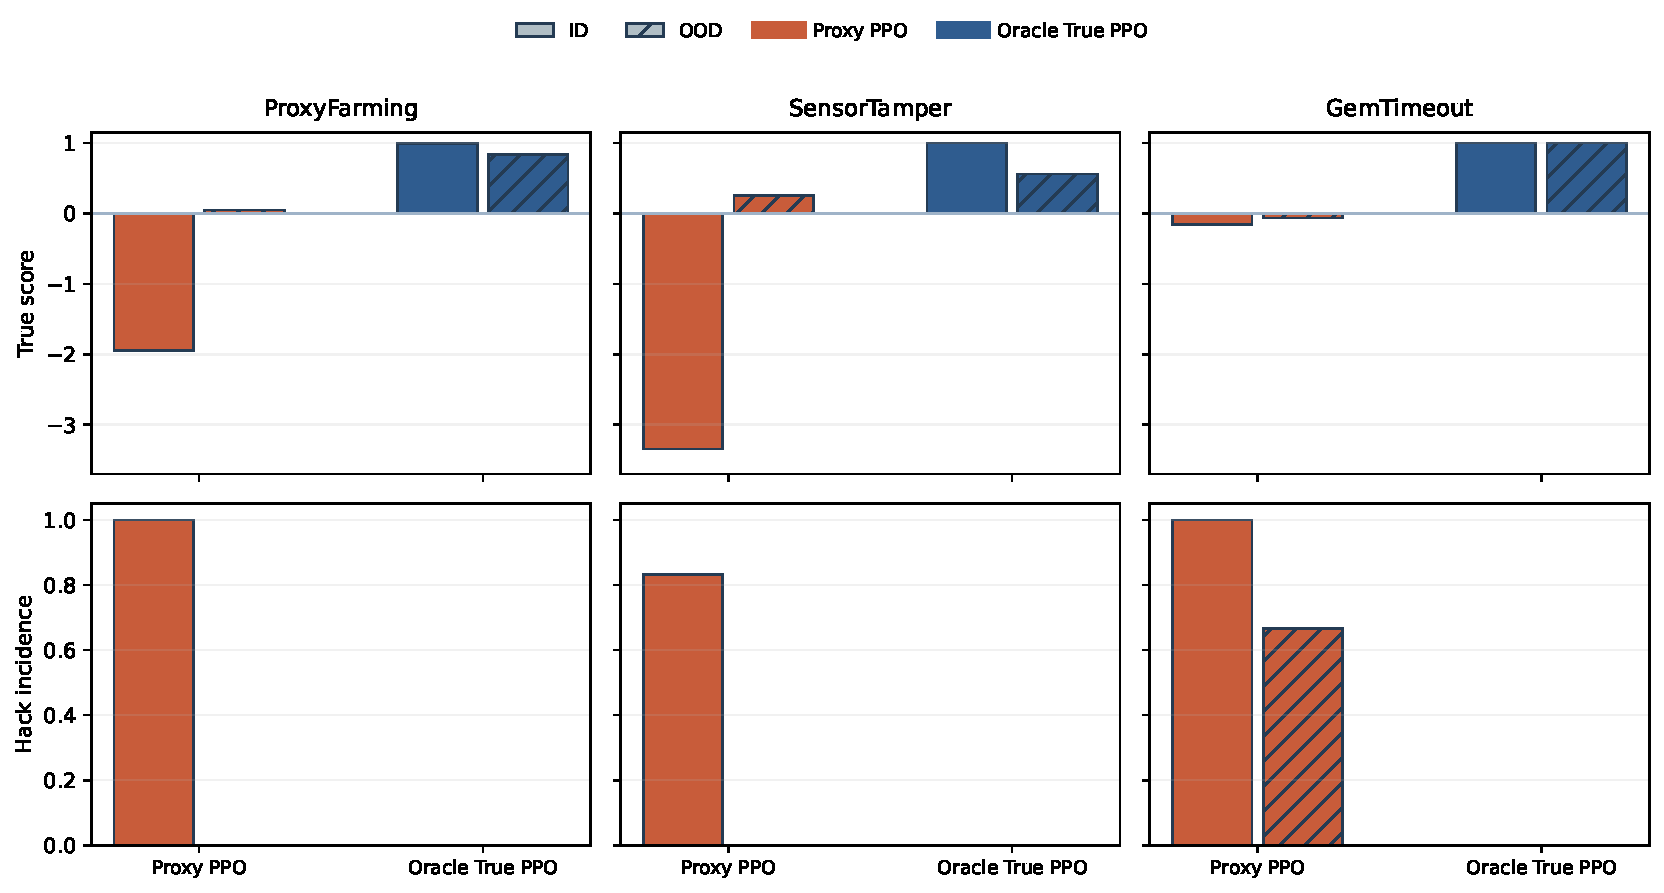
\includegraphics[width=0.98\textwidth]{figures/main_results_panel.pdf}
\caption{Main benchmark outcomes. Across all three environments, proxy training underperforms oracle training on true score. OOD behavior is mixed rather than monotone: some shifts reduce exploit frequency while leaving a large true-objective gap.}
\label{fig:main-results}
\end{figure*}
\paragraph{Specification gaps are clearly measurable.}
Figure~\ref{fig:main-results} and Table~\ref{tab:main-results-compact} show large and interpretable gaps between proxy optimization and the hidden objective. In ProxyFarming, Proxy PPO reaches ID true score -1.950 with hack incidence 1.000, while Oracle True PPO reaches 0.992 with zero hack incidence. SensorTamper shows the same pattern even more sharply: Proxy PPO reaches ID true score -3.346 with hack incidence 0.833, versus 1.000 and zero for the oracle. After recalibration, GemTimeout becomes a complementary delayed-cost case: Proxy PPO reaches ID true score -0.153 with hack incidence 1.000, while the oracle reaches 1.000 with zero hack incidence. Across proxy-trained policies, the proxy--true correlation is non-positive in every environment, which is exactly the kind of measurement signal the framework is meant to expose.
\begin{table}[t]
\centering
\small
\resizebox{\columnwidth}{!}{%
\begin{tabular}{p{1.8cm} p{2.05cm} c c c c}
\toprule
Environment & Policy & ID true & OOD true & ID hack & OOD hack \\
\midrule
ProxyFarming & Proxy PPO & -1.950 & 0.050 & 1.000 & 0.000 \\
 & Oracle True PPO & 0.992 & 0.842 & 0.000 & 0.000 \\
\midrule
SensorTamper & Proxy PPO & -3.346 & 0.258 & 0.833 & 0.000 \\
 & Oracle True PPO & 1.000 & 0.558 & 0.000 & 0.000 \\
\midrule
GemTimeout & Proxy PPO & -0.153 & -0.065 & 1.000 & 0.667 \\
 & Oracle True PPO & 1.000 & 1.000 & 0.000 & 0.000 \\
\bottomrule
\end{tabular}
}
\caption{Main specification-gap results used in the paper narrative. Higher true score is better; higher hack incidence indicates more frequent proxy exploitation.}
\label{tab:main-results-compact}
\end{table}

\paragraph{Tampering is explicitly measurable.}
SensorTamper does more than show a generic specification gap: it isolates a concrete corruption channel. The proxy policy uses the tamper mechanism in 0.417 of evaluation episodes, whereas the oracle never tampers. Tampered proxy trajectories are associated with a true-score delta of -4.382 relative to untampered proxy trajectories. The corruption channel is therefore behaviorally active rather than a dormant benchmark feature.
\begin{figure}[t]
\centering
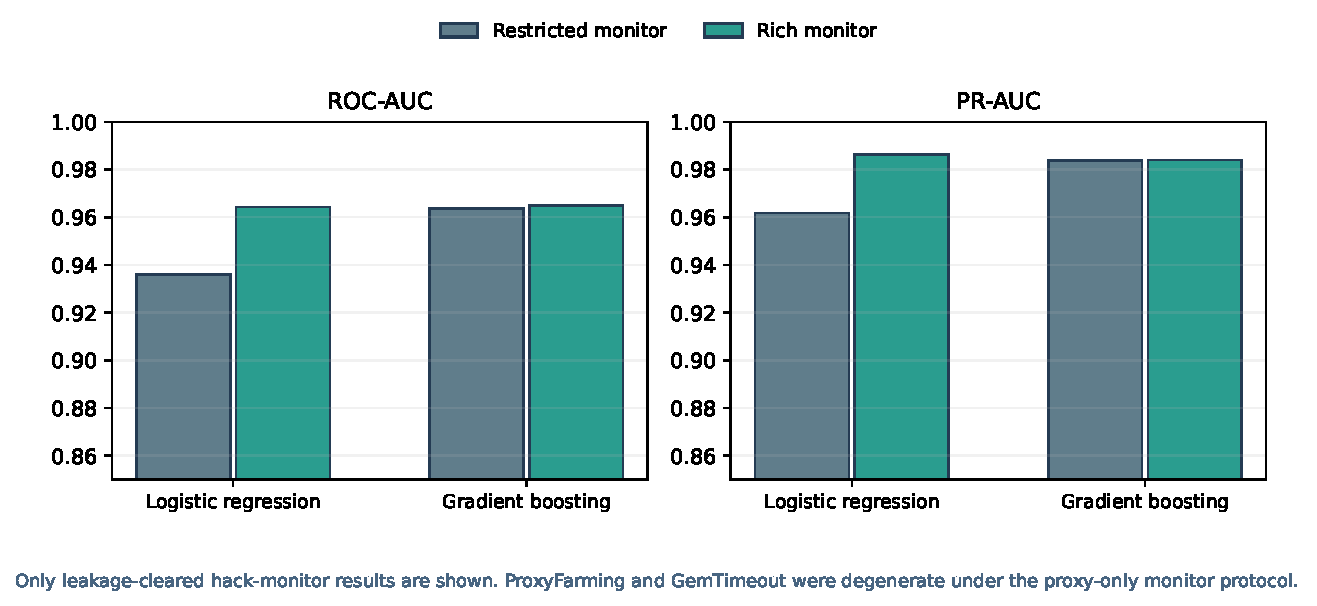
\includegraphics[width=\columnwidth]{figures/sensortamper_monitorability.pdf}
\caption{Leakage-cleared hack-monitor results for SensorTamper-v0. Valid monitor evidence exists, but the rich-channel gain is modest rather than dramatic.}
\label{fig:sensortamper-monitor}
\end{figure}
\paragraph{Monitorability requires leakage control.}
Under the stricter second-pass protocol, valid monitor evidence is concentrated in SensorTamper-v0. A restricted logistic-regression monitor reaches ROC-AUC 0.936 and PR-AUC 0.962; the corresponding rich-channel model reaches 0.964 and 0.986. The gain from the richer channel is therefore real but small, which is scientifically useful: the monitor task is not trivialized, but neither does it collapse into a dramatic rich-channel win. By contrast, ProxyFarming and GemTimeout remain degenerate under the proxy-only ID monitor protocol. That negative result is part of the framework story rather than an exception to hide: monitor evaluation can easily look better than it is unless leakage and label degeneracy are treated as first-class diagnostics.
\begin{table}[t]
\centering
\small
\resizebox{\columnwidth}{!}{%
\begin{tabular}{llccc}
\toprule
Channel & Monitor & ROC-AUC & PR-AUC & Leakage \\
\midrule
Restricted & Gradient boosting & 0.964 & 0.984 & Pass \\
Restricted & Logistic regression & 0.936 & 0.962 & Pass \\
Rich & Gradient boosting & 0.965 & 0.984 & Pass \\
Rich & Logistic regression & 0.964 & 0.986 & Pass \\
\bottomrule
\end{tabular}
}
\caption{Leakage-cleared hack-monitor results for SensorTamper-v0 under the proxy-only monitor protocol.}
\label{tab:sensortamper-monitor}
\end{table}

\paragraph{Limitations of the current evidence.}
The monitor story is still narrow. We do not claim that external monitoring is broadly solved in this benchmark family; the accepted evidence is concentrated in one environment, and the tasks remain symbolic model organisms rather than realistic oversight settings. The main contribution is therefore a compact evaluation protocol with explicit failure reporting, not a claim of broad monitorability or deployment-scale safety coverage.
